\section{Matrix-Vector Multiplication}%

\textbf{This part might be too easy for most of you - but it would still give you intuition in the contents we would discuss later.} From the master notes we are given that:
\[
x = \begin{pmatrix} x_1\\x_2\\ \vdots\\ x_n \end{pmatrix} \text{, and } x \in \mathbb{C}^{n}
.\]
and
\[
  A = \begin{pmatrix} 
  a_{11} & a_{12} & \ldots & a_{1n} \\
a_{21} & a_{22} & \ldots & a_{2n} \\ 
\vdots & \vdots & \ddots & \vdots \\
a_{m1} & a_{m2} & \ldots & a_{mn} \\  
\end{pmatrix} 
.\] 
And we are asked to consider the matrix multiplication $b = Ax$:
\begin{itemize}
  \item The first thing we could confirm is $b \in \mathbb{C}^{m}$ by dimensions of the given matrices.
  \item Then speaking about the $i$th component of $b$, $b_i$ (\textbf{obviously, $1 \le i \le m$}), how do we determine the value of $b_i$ in general? 
  \item Normally we get the $i$th row from our matrix $A$, and multiply with the column vector $x$ using matrix multiplication rules:
    \[
    b_i = a_{i1}x_1 + a_{i2}x_2 + \ldots +  a_{in}x_n = \sum_{j = 1}^{n} a_{ij}x_j
    .\]
  where $i \in \{1, 2, 3 \ldots m\}$.
    \item This is what we called Matrix-Vector multiplication. And as the master notes saying, we could check the map $x \to  Ax$ given by matrix multiplication is a linear map from $\mathbb{C}^{n} \to \mathbb{C}^{m}$. We need to show that:
      \[
        \forall x, y \in \mathbb{C}^{n}, \alpha \in \mathbb{C}, A(\alpha x + y) = \alpha A x + A y
      .\]
    \item This should be really straightforward.
\end{itemize}
\subsubsection*{Proof}
\begin{itemize}
    \item Suppose $b = A(\alpha x + y)$, we compute the $i$th entry of $b$,  $b_i = [A(\alpha x + y)]_{i}$ via the formula above:
      \[
        b_i = \sum_{j = 1}^{n} a_{ij}(\alpha x + y)_j =  \sum_{j = 1}^{n} a_{ij}(\alpha x_j + y_j)
      \]
      \[
        = \alpha(\sum_{j = 1}^{n} a_{ij} x_j) + (\sum_{j = 1}^{n} a_{ij} y_{j})
      .\]
    \item Can you see that how could we simplify this expression further? Use the Matrix-Vector formula we derived before:
      \[
        b_i = \alpha (Ax)_i + (Ay)_i
      \]
    \item Therefore, sub in $b_i = [A(\alpha x + y)]_i$ into the equation we have:
      \[
        [A(\alpha x + y)]_i = \alpha (Ax)_i + (Ay)_i
      \]
      \[
        \implies A(\alpha x + y) = \alpha Ax + Ay
      .\]
    \item Therefore, we could now confirm that the map $x \to Ax$ by multiplication is a linear map.
    \item You have now seen the derivation of Matrix-Vector Multiplication formula and its property, but how do we implement this schema as a python function? Try Exercise 1.1!
\end{itemize}

\subsection*{Exercise 1.1: Basic M-V Multiplication}%
\addcontentsline{toc}{subsection}{Exercise 1.1: Basic M-V Multiplication}
\subsubsection*{Problem Description}
In this exercise, we are given matrix $A$ and vector $x$ as defined above. What we need to is implementing a function which returns the matrix-vector product $b = Ax$. We are asked to implement this with a \textbf{double-nested loop}.

\smallskip
\noindent How do we implement this function? 

\begin{itemize}
  \item Since this is the very first exercise, I would show you the mathematics behind the implementation, the steps you need to do in the implementation, and how to translate steps into code, in details. 
  \item \textbf{Note: Detailed explanation/analysis about how to write code would only be in this exercise, but would not be provided in any future exercises.}
\end{itemize}
\subsubsection*{What to do}
\begin{enumerate}
    \item Think about the formula we derived in the previous section:
    \[
    b_i = \sum_{j = 1}^{n} a_{ij} x_j, i \in \{1, 2, 3 \ldots m\}
    .\] 
  \item There is a summation sign in the caclulation of $b_i$, and it should indicate a \textbf{for} loop in the implementation of calculating $b_i$.
  \item \textbf{Note: We always relate the summation in mathematics and for loop in programming together, try to convince yourself that you really understand why we were allowed to do so.}
  \item Also the basic 'algorithm' indicates that we would compute the value of $b_i$ for $m$ times, with similar methods. Therefore, there should be another \textbf{for} loop to compute all values of $b_i$ in $m$ iterations. Now you should understand why a \textbf{double-nested for loop} is necessary for our implementation.
\end{enumerate}
\begin{itemize}
   \item Therefore, the structure of our implementation should be:
     \lstinputlisting[language=Python, firstline=1, lastline=14]{./python/exercise1.py}
\end{itemize}
\subsubsection*{Analysis}
    \begin{itemize}
    \item Then the implementation has been divided into two parts: compute the values of $b_i$ through the inner loop iterations, and add these values to the placeholder, a list $b$ as each inner loop ends.
    \item The second part is very easy to implement, just append the computed $b_i$ to $b$ via \texttt{b.append(bi)} at the end of each iteration of the outer loop.
    \item The first part is still straight-forward, but would take more effort in the implementation. To compute the value of $b_i$, we should initialize the value as 0 at first, i.e. \texttt{bi = 0}. Then we could go into the inner loop with counter $j$ to do the summation. 
    \item Then the 'elements' we need in the inner loop is kind of self-intuitive, since it is mentioned in the basic formula:
      \[
        \sum_{i = 1}^{n} \to \texttt{for j in range(n)}
      \] 
       \[
         a_{ij} \to  \texttt{A[i, j]}
      \] 
      \[
        x_j \to  \texttt{x[j]}
      .\]     
    \item Since we are doing summation, what we are going to do in the inner loop is just to keep adding computed results during iterations of $j$, i.e.  \texttt{bi += A[i][j] * x[j]} in each iteration of $j$.
    \item The function requires an n-dimentional \texttt{ndarray}, so we need to wrap the list \texttt{b} with \texttt{np.array()} when function returns the result.
  \end{itemize}
\subsubsection*{Code Implementation} 
\begin{itemize}
    \item Therefore, we have all things we need from analysis above, and fill the template we would get the final implementation:
      \lstinputlisting[language=Python, firstline=17, lastline=33]{./python/exercise1.py}
    \item \textbf{(Important!)} To test your code, do not forget to activate your virtual environment first, and then using either \texttt{pytest} or \texttt{py.test} to do the testing.
    \end{itemize}
\section{Column-Space Formulation}
In this section, we would give you an intuition to interpret matrix-vector multiplication as a linear combination of columns of $A$, with coefficients taken from the entries of $x$.
 \begin{itemize}
\item If we write the result of $b = Ax$ explicitly, we would get:
\[
b = \begin{pmatrix} a_{11}x_1 + a_{12}x_2 + \cdots + a_{1n}x_n \\  a_{21}x_1 + a_{22}x_2 + \cdots + a_{2n}x_n\\ \vdots\\a_{m1}x_1 + a_{m2}x_2 + \cdots + a_{mn}x_n \end{pmatrix}
\]
\[
 = x_1\begin{pmatrix} a_{11}\\ a_{21} \\ \vdots\\ a_{m1} \end{pmatrix} + x_2 
\begin{pmatrix} a_{12}\\ a_{22} \\ \vdots\\ a_{m2} \end{pmatrix} + \cdots + x_n 
\begin{pmatrix} a_{1n}\\ a_{2n} \\ \vdots\\ a_{mn} \end{pmatrix}
.\]
which is a linear combination with columns of $A$ and entries of $x$.
 \item To simplify this more, we could rewrite matrix $A$ in terms of all of its columns as follows:
    \[
   A = \begin{pmatrix}
     a_1 & a_2 & \ldots & a_n
   \end{pmatrix}
   .\]
   where
   \[
   a_i = \begin{pmatrix} a_{1i}\\ a_{2i} \\  \vdots\\ a_{mi} \end{pmatrix} \in \mathbb{C}^{m}, i \in \{1, 2, \ldots n\} 
   .\]
  \item Therefore, the linear combination should be:
     \[
    b = x_1a_1 + x_2a_2 + \cdots + x_na_n = \sum_{j=1}^{n} x_j a_j
    .\] 
\end{itemize}
\subsection*{Exercise 1.2: M-V Multiplication with C-S Formulation}%
\addcontentsline{toc}{subsection}{Exercise 1.2: M-V Multiplication with C-S Formulation}
\subsubsection*{Problem Description}
The question says the given conditions are unchanged. However, in this implementation we were asked to \textbf{use a single loop} over entries of A (and x).

\medskip
\noindent So considering the column-space formulation we mentioned above, we could easily get the implementation by using:
\[
b = Ax =  \sum_{i=1}^{n} x_i a_i
.\]

\subsubsection*{Code Implemenation}
\lstinputlisting[language=Python, firstline=36, lastline=46]{./python/exercise1.py}
\subsubsection*{Analysis} 
Here are several things also worth mentioning:
\begin{itemize}
\item Since we are asked to use a \textbf{single loop} only, we could easily see that using the formula with one $\Sigma$ sign would work. i.e. the formula with column-space formulation.
\item Then according to the formula derivation above, we only need to iterate through the column vectors in matrix $A$, i.e. \texttt{A[:, i]} and multiply with the $i$th entry of $x$, the final result would be calculated as the sum of products in each iterations.
\item The placeholder of the result, \texttt{b}, is initialized as a \texttt{numpy} array with zeros, rather than an empty array. 
\item That is because in the addition of numpy, two arrays should be equi-dimentioned. Using an empty array would make the dimension zero, which is obviously different from the dimension of product obtained in each iteration.
\item I used \texttt{for i, elem in enumerate(x)} in my implementation, rather than \texttt{for i in range(len(x))} and \texttt{elem = x[i]} for code simplicity and elegance.
\end{itemize}
\section{Matrix-Matrix Multiplication}%
\textbf{This part of derivation is similar to the Matrix-Vector case.} Now our matrix $A$ is in dimension $\mathbb{C}^{m \times l}$, and consider another matrix $C \in \mathbb{C}^{l \times n}$ and we have matrix $B = AC$:
\begin{itemize}
  \item Then we think about the entry $(i, j)$ of matrix $B$. To get the value of $b_{ij}$, we should get the $i$th row from $A$ and the $j$th column from $C$, and the calculation goes like this:
    \[
      b_{ij} = a_{i1}c_{1j} + a_{i2}c_{2j} + a_{i3}c_{3j} + \ldots +  a_{il}c_{lj} = \sum_{k = 1}^{l} a_{ik}c_{kj}
    .\] 
    where
    \[
      (i, j) \in \{1, 2, 3 \ldots m\} \times \{1, 2, 3 \ldots n\} 
    .\]
    \item Now we have seen the derivation of formula of matrix multiplication, in different cases.
    \item Then try to apply the column-space formulation to the matrix-matrix multiplication, considering the $i$th column of the result matrix, $b_i$, the column vector is obtained via:
    \[
    b_i = A c_i
    .\] 
    which is another product of matrix-vector multiplication.
    \item Therefore, we expand the matrix-vector multiplication and we could get:
    \[
    b_i = \sum_{j=1}^{l} A_j c_{ij}
    .\]
    for a matrix-matrix multiplication with column-space formulation.

\end{itemize}
\subsection*{Exercise 1.3: Execution Time Comparison}%
\addcontentsline{toc}{subsection}{Exercise 1.3: Execution Time Comparison}
\subsubsection*{Problem Description}
In this section we are not asked to implement anything, but we could use the defined function $\texttt{time\_matvecs()}$ in package to see the different execution time, for different matrix multiplication algorithm implementations:
\begin{lstlisting}
> basic_matvec(A0, x0) # double-nested loop implementation

> column_matvec(A0, x0) # single loop implementation

> A0.dot(x0) # numpy implementation
\end{lstlisting}
\subsubsection*{Efficiency Measuring}
Here we compare three implementations mentioned above, and the timing function gives us the following results:
\begin{lstlisting}
>>> import cla_utils
>>> cla_utils.time_matvecs()
Timing for basic_matvec
0.09208189499999975
Timing for column_matvec
0.002095079000000055
Timing for numpy matvec
0.00014622799999841618
\end{lstlisting}
We would clearly see the execution time:
\[
\texttt{nested loop} \gg \texttt{single loop} \gg \texttt{numpy implementation}
.\]
As the master notes saying, in these exercises you should consider the best way to \textbf{make use of Numpy built-in operations} (which will often make the code more maths-like and readable, as well as potentially faster).
\section{Range of a Matrix}%
The master notes have the definition of \texttt{range}, here I would give the definition in set notation \textbf{(alternative version of Definition 1.4 master notes)} :
\[
\text{range}(A) = \{a : \exists x \in \mathbb{C}^{n}, Ax = a \}, \text{ where } A \in \mathbb{C}^{m \times n}
.\]
Here we would see any $a \in A$ would be expressed as a product in form of M-V multiplication. In other words, we could manipulate $a$ as a product with column-space formulation, with the following interpretation:
\[
a = Ax = \sum_{i=1}^{n} A_i x_i
.\]
Therefore, any element in range($A$) could be demonstrated as a \textbf{linear combination} of \textbf{column vectors} in A. In other words, \textbf{any element $a \in \text{range}(A)$ would be in the vector space spanned by column vectors of $A$.} So we have the following statement:
\[
  \forall a \in \text{range}(A), a \in \text{span}(a_1, \cdots, a_n) \implies \text{range}(A) \subseteq \text{span}(a_1, \cdots, a_n)
.\] 
Also we could see that, \textbf{any linear combination} of columns of $A$ is an element of range$(A)$, which means:
\[
  \forall v \in \text{span}(a_1, \cdots, a_n), v \in \text{range}(A) \implies \text{span}(a_1, \cdots, a_n) \subseteq \text{range}(A)
.\] 
Therefore, we finally have:
\[
  \text{range}(A) = \text{span}(a_1, \cdots, a_n)
.\] 
That is to say, range($A$) is the vector space spanned by the columns of $A$, as mentioned in the  \textbf{Theorem 1.5} of master notes. 

\section{Null Space and Rank of a Matrix}%
The definition of the null space of an Matrix is very simple as stated by the master notes:
\[
  \text{null}(A) = \{x \in \mathbb{C}^{n}: Ax = 0\} 
.\]
Then we would talk about the rank of a matrix. Actually we have two definitions, \textbf{row rank} and \textbf{column rank}, which refer to the dimension of the row/column space. It could be shown that these two values are equal for all matrices, here is the proof:
\subsubsection*{Proof}
\begin{itemize}
  \item Suppose we have a matrix $A \in \mathbb{C}^{m \times n}$, and we could put this matrix into its RRE form, $A'$, by elementary row operations (an example is given below, where $a'_{in} \neq 1$):
  \[
    A' = \begin{pmatrix}
    1 & a'_{11} & 0 & a'_{14} &  \cdots & 0 & 0 & 0 & \cdots & 0\\
    0 & 0 & 1 & a'_{23} & \cdots & 0& a'_{2n} & 0 & \cdots & 0\\
    0 & 0 & 0 & 0 &  \cdots & 1 & a'_{3n} & 0 & \cdots & 0\\
    \vdots & \vdots & \vdots & \vdots & \vdots &\vdots & \vdots & \vdots & \vdots & \vdots \\
    0 & 0 & 0 & 0 & \cdots & 0 & 0 & 0 & \cdots & 0
    \end{pmatrix} 
  .\]
  \item Similarly, we could put $A'$ into its column reduced form,  $A''$. Since the elementary row and column operations are both invertible. That is to say, there exists two invertible matrices  $P$ and  $Q$, such that:
   \[
  QPA = A''
  .\] 
  and since $P$ and $Q$ are invertible, the number of linearly independent row (\textbf{also for column}) vectors in  $A''$ should be equal to the number in $A$.
  \item Now $A''$ is in both row reduced and column reduced form, so $A''$ should be in the following form:
   \[
  A'' = \begin{pmatrix} 
  I_k & 0_{k \times  (n - k)} \\
  0_{(m - k) \times k} & 0_{(m - k) \times (n - k)}
  \end{pmatrix}
  .\]
  \item To be more specific, we could see the structure of $A''$ after the elementary row and column operations through the following figure:
  \begin{figure}[H]
    \centering
    \captionsetup[subfigure]{justification=centering}
      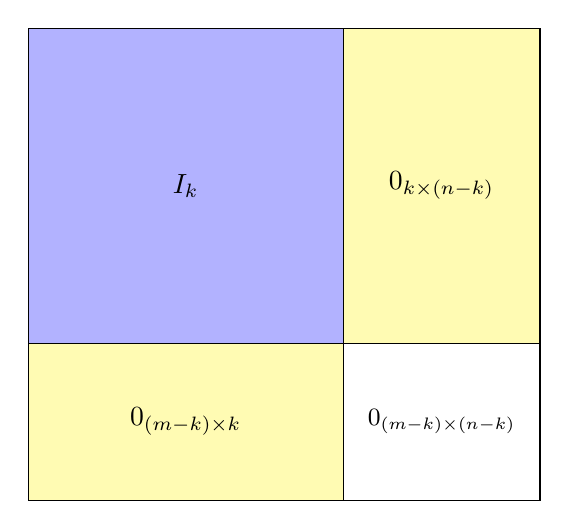
\begin{tikzpicture}
        \filldraw[fill=blue!30!white] (0, 0) rectangle (4, 4) node[pos=.5] {$I_{k}$};
        \filldraw[fill=yellow!30!white] (0, 0) rectangle (4, -2) node[pos=.5] {$0_{(m - k)\times k}$};
        \filldraw[fill=yellow!30!white]  (4, 0) rectangle (6.5, 4) node[pos=.5] {$0_{k\times (n - k)}$};
        \draw (4, 0) rectangle (6.5, -2) node[pos=.5] {\small $0_{(m - k)\times (n - k)}$};
      \end{tikzpicture}
      \caption{Structure of matrix after elementary row and column operations}
  \end{figure}
  \item Then it is not hard to see that, since apart from the identity matrix block $I_k$, the other blocks in $A''$ are just 0s, so the dimension of row space and column space are both equal to the 'size' of the identity matrix block $k$. i.e. the row rank and the column rank are equal for all matrices.
\end{itemize}
Here we have seen the equality of row and column ranks, so as the mater notes saying, we just refer to the rank in this course. By using the definition of range and column space of matrix, for all matrix $A \in \mathbb{C}^{m \times  n}$, we have:
\[
  \text{rank}(A) = \text{dim}(\text{span}(a_1, a_2, \cdots, a_n)) = \text{dim}(\text{range}(A))
.\] 
And I would say the definition of \textbf{full rank} is still straightforward though. However,  to understand it in a more direct (or say 'geometrical') way using the similar intuition from the proof of equality of ranks. So here are two figures to demonstrate of the idea:
\subsubsection*{Demonstration}
\begin{figure}[H]
  \centering
  \captionsetup[subfigure]{justification=centering}
  \begin{subfigure}[b]{0.5\textwidth}
    \centering
    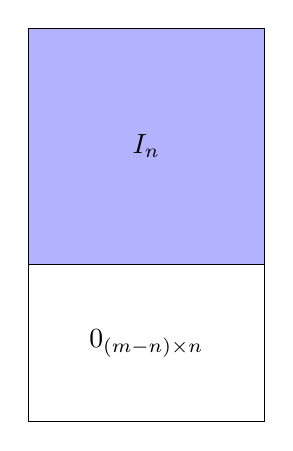
\begin{tikzpicture}
      \filldraw[fill=blue!30!white] (0, 0) rectangle (3, 3) node[pos=.5] {$I_{n}$};
      \draw (0, 0) rectangle (3, -2) node[pos=.5] {$0_{(m - n)\times n}$};
    \end{tikzpicture}
    \caption{$m \ge n$}
    \end{subfigure}
    \hfill
    \begin{subfigure}[b]{0.4\textwidth}
      \centering
      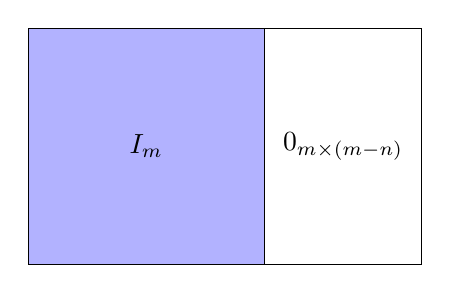
\begin{tikzpicture}
        \filldraw[fill=blue!30!white] (0, 0) rectangle (3, 3) node[pos=.5] {$I_{m}$};
        \draw (3, 0) rectangle (5, 3) node[pos=.5] {$0_{m\times (m - n)}$};
      \end{tikzpicture}
      \caption{$m < n$}
    \end{subfigure}
    \caption{Full rank demonstration}
\end{figure}
\begin{itemize}
  \item Firstly we could think the case $m \ge n$, here $n$ is the 'lesser' in dimension $\mathbb{C}^{m \times n}$, and for the given matrix $A$, the maximum number of linearly independent vectors in column vectors the matrix should be $n$. 
  \item And if we try to continuously do elementary row and column operations like we do in the previous proof, we would get the transformed matrix $A'$. If all column vectors are linearly independent, unlike any general matrix after transformation (see \textbf{Figure 1}), the size of identity matrix block in $A'$ would just fit the 'width' of $A'$($A$ as well), as shown in \textbf{Figure 2(a)}. 
  \item So the rank of matrix $A$, i.e. the size of identity matrix block in $A'$, should be $n$. And the rank cannot be any bigger for all matrix $M \in \mathbb{C}^{m \times n}$. Therefore, we call matrix $A$ has \textbf{full} rank in this case.
  \item In the other case where $m < n$, we could use same intuition to demonstrate the idea of  \textbf{full rank} where the 'lesser' here is the 'height' of $A$, i.e.  $m$ in this case. You could see it from \textbf{Figure 2(b)}.
\end{itemize}
\section{Full Rank and Matrix Properties}%
In this part, we are going to talk about the proof of  \textbf{Theorem 1.9} in the master notes:
\[
  \forall A \in \mathbb{C}^{m \times n}, A \text{ full rank} \iff \neg (\exists x, y \in \mathbb{C}^{n}, x \neq  y \implies Ax = Ay)
\]
\[
  \iff (\forall x, y \in \mathbb{C}^{n}, x \neq y \implies Ax \neq Ay) \iff A \text{ is an injection}
\]
\[
\iff \forall x \in \mathbb{C}^{n} Ax \text{ is unique in }\mathbb{C}^{m}
.\] 
\subsubsection*{Proof}
\begin{itemize}
  \item Without loss of generality, we consider the case that $m \ge  n$.
  \item \textbf{To prove the forward proposition}, we could use the column-space formulation in multiplication $Ax$ and have:
     \[
    Ax = \sum_{i=1}^{n} x_i a_i
    \]
    with $a_i$ represents the  $i$th column of matrix $A$.
  \item Since $A$ is full rank, so all column vectors are linearly independent. Therefore, $Ax$ gives out a unique linear combination in  $\mathbb{C}^{m}$ formed by columns of $A$. i.e. no two distinct vectors would be mapped to same vector, so the forward direction has been proved.
  \item \textbf{To prove the backward proposition}, we use the Rank-Nullity theorem, for any given linear map $T: V \to  W$, where $V, W$ are vector spaces and  $V$ is finite dimensional:
    \[
      \text{rank}(T) + \text{nullity}(T) = \text{dim}(V)
    .\]
  \item Since $A : \mathbb{C}^{n} \to  \mathbb{C}^{m}$, we have $\text{dim}(A) = n$.
  \item Considering $\text{nullity}(A) = \text{dim}(\text{null}(A))$, since for null$(A)$:
    \[
      \text{null}(A) = \{x \in \mathbb{C}^{n}: Ax = 0_m\} 
    .\]
  \item Since $A$ cannot be a zero matrix, so the only vector could satisfy $Ax = 0_m$ should be  $x = 0_n$. i.e. 
    \[
      \text{null}(A) = \{0_n\} \text{ and nullity}(A) = \text{dim}(\{0_n\}) = 0
    .\]
  \item Therefore, according to Rank-Nullity theorem, we have 
    \[
      \text{rank}(A) = n - 0 = n = \text{min}(m, n)
    .\]
  \item So we could prove A is full rank, and we have done proofs of both forward and backward propositions.
  \item We could do the same thing for the case $m < n$, and just as the master notes saying, the theorem is a consequence of the column space interpretation of matrix-vector multiplication.

\end{itemize}
And also it is clear to see the relations between the full rank and invertibility of an matrix, nothing added for explaining \textbf{Theorem 1.10}.
\subsection*{Exercise 1.11: Construct a Rank-2 Matrix}%
\addcontentsline{toc}{subsection}{Exercise 1.11: Construct a Rank-2 Matrix}
\subsubsection*{Problem Description}
Given that we have $u_1, u_2 \in \mathbb{C}^{m}$ and $v_1, v_2 \in \mathbb{C}^{n}$, we want to construct a rank-2 matrix $A = u_1v_1^{*} + u_2v_2^{*}$. However, from the given code and the specification, we need to somehow return matrix  $A$ as a product of two other matrices $B$ and $C$.
\subsubsection*{What to do}
We need to consider the following two questions:
\begin{itemize}
  \item How to write $A$ in terms of a product of matrices?
  \item Why $A$ is rank-2 under this construction?
\end{itemize}
And here we consider the $A$ as a summation of two matrices first:
\[
A = u_1v_1^{*} + u_2v_2^{*}
\]
where
\[
  u_1v_1^{*} = \begin{pmatrix} v_{11}^{*}u_1 & v_{12}^{*}u_1 & \cdots & v_{1n}^{*}u_1 \end{pmatrix} 
\]
and
\[
  u_2v_2^{*} = \begin{pmatrix} v_{21}^{*}u_2 & v_{22}^{*}u_2 & \cdots & v_{2n}^{*}u_2 \end{pmatrix} 
.\] 
Therefore, $A$ could be written in the sum:
\[
  A = u_1v_1^{*} + u_2v_2^{*} = \begin{pmatrix} v_{11}^{*}u_1 + v_{21}^{*}u_2 & v_{12}^{*}u_1 + v_{22}^{*}u_2 & \cdots & v_{1n}^{*}u_1 + v_{2n}^{*}u_2 \end{pmatrix} 
\]
with
\[
  a_{i} = v_{1i}^{*}u_1 + v_{2i}^{*}u_2 = \begin{pmatrix} u_1 & u_2 \end{pmatrix} \begin{pmatrix} v_{1i}^{*}\\ v_{2i}^{*} \end{pmatrix}
.\] 
To generalize this, we could now write $A$ in terms of a product of two matrices:
\[
A = \begin{pmatrix} u_1 & u_2 \end{pmatrix} \begin{pmatrix} v_{1}^{*}\\ v_{2}^{*} \end{pmatrix}  
.\]
So our first job has been done, now here is the implementation:
\subsubsection*{Code Implementation}
\lstinputlisting[language=Python, firstline=56, lastline=69]{./python/exercise1.py}
Now let us talk about the rank of $A$, why it is necessarily 2?
We recall the result of $A$ we have found with column-space formulation: 
\[
A = u_1v_1^{*} + u_2v_2^{*} = \begin{pmatrix} v_{11}^{*}u_1 + v_{21}^{*}u_2 & v_{12}^{*}u_1 + v_{22}^{*}u_2 & \cdots & v_{1n}^{*}u_1 + v_{2n}^{*}u_2 \end{pmatrix} 
.\]
We could see that, every column of $A$ is a linear combination of $u_1$ and $u_2$, assume that they are linearly independent. Therefore, when we are talking about the range of $A$, it should be a vector space spanned by $u_1$ and $u_2$ and the dimension of the space should be 2. \textbf{i.e. the rank is 2 obviously.} 
\newpage
\section{Invertibility and inverses}%
The idea and properties related to invertibility and inverses should be quite familiar, I would not talk about this here. What I want to focus is the proof exercise mentioned in the master notes, and the exercise in this part.
\subsubsection*{Problem Description}
The exercise is asked us to prove that, there exists a unique \textbf{left} inverse $Z$ of a given square matrix $A \in \mathbb{C}^{n \times n}$ such that $ZA = I_n$. And here is the proof:
\subsubsection*{Proof}
\begin{itemize}
  \item Suppose there exists another left inverse $Z'$ of $A$, such that  $Z'A = I_n$ but  $Z' \neq  Z$.
  \item Consider the $(i, j)$ entry of the product $Z'A$, if $i \neq j$:
    \[
      (Z'A)_{ij} = \sum_{k=1}^{n} z'_{ik}a_{kj} = 0
    \]
    and similarly
    \[
      (ZA)_{ij} = \sum_{k=1}^{n} z_{ik}a_{kj} = 0
    .\]
  \item Therefore, we subtract one equation from another, we would have:
    \[
      (ZA)_{ij} - (Z'A)_{ij} = \sum_{k=1}^{b} (z_{ik} - z'_{ik})a_{kj} = 0 - 0 = 0
    .\]
  \item The sum equals zero indicates that, when $i \neq  j$, for all $k$, the non-trivial case would give us:
     \[
    z_{ik} - z'_{ik} = 0 \implies z_{ik} = z'_{ik}
    .\] 
  \item Similarly, when $i = j$, we would know that  $(Z'A)_{ij} = (ZA)_{ij} = 1$. So after subtraction like we did above, we would get:
    \[
      (ZA)_{ij} - (Z'A)_{ij} = \sum_{k=1}^{b} (z_{ik} - z'_{ik})a_{kj} = 1 - 1 = 0
    .\]
    and again
    \[
    z_{ik} - z'_{ik} = 0 \implies z_{ik} = z'_{ik}
    .\] 
  \item Therefore, we have seen $z_{ik} = z'_{ik}$ in each scenario, therefore, our suggested new left inverse $Z'$ is just original $Z$ itself, which gives a contradiction.
   \item So we have now proved the left inverse is unique.
  \item We could use the same strategy to prove the uniqueness of right inverse $Z$ such that  $AZ = I_n$.
  \item Therefore, we could say the inverse $Z$, of a square matrix $A$, such that  $ZA = AZ = I_n$, is unique if the matrix itself is invertible.
\end{itemize}
\subsection*{Exercise 1.13: Find the inverse of a given matrix}%
\addcontentsline{toc}{subsection}{Exercise 1.13: Find the inverse of a given matrix}
\subsubsection*{Problem Description}
Given that a square matrix $A = I_m + uv^{*} \in \mathbb{C}^{m \times m}$, where $u, v \in \mathbb{C}^{m}$. Suppose we could find the inverse $A'$ written in  $A' = I_m + \alpha uv^{*}$, determine the value of $\alpha$ and implement the function $\texttt{rank1pert\_inv()}$ to return the inverse matrix $A'$.
So we try to determine the value of $\alpha$ first:
\subsubsection*{Analysis}
\begin{itemize}
  \item Given that $A A^{-1} = I_m$:
    \[
      A A^{-1} = (I_m + u v^{*})(I_m + \alpha u v^{*}) = I_m + uv^{*} + \alpha uv^{*} + \alpha u v^{*}uv^{*} = I_m
    .\]
  \item From the numerical analysis course we know the inner product, $v^{*}u$ is a scalar, then we could have:
    \[
      uv^{*} + \alpha uv^{*} + \alpha (v^{*}u)uv^{*} = 0_{m \times m} \implies (1 + \alpha + \alpha v^{*}u)uv^{*} = 0_{m \times m}
    .\]
  \item Therefore, we have:
    \[
    \alpha (1 + v^{*}u) = -1 \implies \alpha = -\frac{1}{1 + v^{*}u}
    \]
    and
    \[
    A^{-1} = I_m -\frac{1}{1 + v^{*}u} uv^{*}
    \]
    whenever $A$ is invertible.
\end{itemize}
So the code implementation shoule be very simple.
\subsubsection*{Code Implementation}
\lstinputlisting[language=Python, firstline=72, lastline=79]{./python/exercise1.py}
\subsubsection*{Efficiency Measuring}
To measure the time taken for computing inverse of this implementation, and compare it with the built-in numpy implementation (just like what we did for timing the matrix-vector multiplication), I add the following code:
\lstinputlisting[language=Python, firstline=82, lastline=100]{./python/exercise1.py}
and the output shows that:
\begin{lstlisting}
>>> import cla_utils
>>> cla_utils.time_matinvs()
Timing for basic_matinv
0.0013024520000044504
Timing for numpy matinv
0.005589449000012792
\end{lstlisting}

\noindent We could see that the numpy implementation is slower. The reason of this output I suppose is that, the complexity of the numpy implementation, to be more specific, the number of operations in the numpy implementation is more than that in our implementation above. Therefore, it takes longer time to compute the inverse.

\section{Adjoints and Hermitian Matrices}%

We firstly skip the definition of adjoints and Hermitian matrices since they are straightforward enough. Then we see the proof of \textbf{theorem 1.15}, which states:
\[ 
  (AB)^{*} = B^{*}A^{*}, A \in \mathbb{C}^{m \times n}, B \in \mathbb{C}^{n \times l}
.\] 
And the proof should be simple.
\subsubsection*{Proof}
\begin{itemize}
  \item Considering the $(i, j)$ entry of $(AB)^{*}$ and we have:
    \[
      (AB)^{*}_{ij} = \overline{(AB)_{ji}}=\overline{\sum_{k=1}^{n} a_{jk}b_{ki}} = \sum_{k=1}^{n} \overline{a_{jk}b_{ki}} = \sum_{k=1}^{n} \overline{a_{jk}}\overline{b_{ki}}
    \]
    \[
      = \sum_{k=1}^{n} (a^{*})_{kj} (b^{*})_{ik} = \sum_{k=1}^{n} (b^{*})_{ik} (a^{*})_{kj} = (B^{*}A^{*})_{ij}
    .\]
  \item Therefore, we finally have $(AB)^{*} = B^{*}A^{*}$.
\end{itemize}
And then we could look at the following exercise implementing the required function \texttt{ABiC()}.
\subsection*{Exercise 1.16: Hermitian Matrices and Multiplication}%
\addcontentsline{toc}{subsection}{Exercise 1.16: Hermitian Matrices and Multiplication}
This exercises have several mini-questions for us to solve. The first part is mainly about proof with hermitian matrices, and the function implementation part is about the application. Let's see the proof exercise first.

\subsubsection*{Task 1}%

\noindent Given that $A = B + iC \in \mathbb{C}^{m \times m}$ where $B, C$ are both real matrices with compatible dimensions, and  $A$ is hermitian, show that:
\[
  B = B^{T} \text{ and } C = -C^{T}
.\]
\subsubsection*{Proof}
\begin{itemize}
  \item Given that $A$ is hermitian then the property tells us:
    \[
      A = A^{* } \text{ with } a_{ij} = (a^{*})_{ij} = \overline{a_{ji}}
    .\]
  \item Considering the $ (i, j)$ and $(j, i)$ entries of $A$, we have:
    \[
    a_{ij} = b_{ij} + ic_{ij} \text{ and } a_{ji} = b_{ji} + ic_{ji}
    .\] 
  \item Therefore, since $A$ is hermitian, we have:
    \[
    a_{ij} = \overline{a_{ji}} \implies b_{ij} + ic_{ij} = \overline{b_{ji} + ic_{ji}} = b_{ji} - ic_{ji}
    .\] 
  \item Clearly
    \[
    b_{ij} = b_{ji} \text{ and } c_{ij} = -c_{ji}
    .\]
  \item Therefore,
    \[
    B = B^{T} \text{ and } C = -C^{T}
    .\] 
\end{itemize}
\subsubsection*{Task 2}%
We required to compute the real and imaginary part of the matrix multiplication product $z = Ax$, where  $A$ is defined above. To save memory the function would accept the contents of $A$ as an argument, but a modified matrix $\hat{A}$, where
\[
\hat{A}_{ij} = \left\{
  \begin{array}{l}
  B_{ij} \text{ where } i \ge j \\
  C_{ij} \text{ where } i < j.
  \end{array}
\right.
.\] 
Therefore, given a matrix $\hat{A}$ and $x_r, x_i$ where  $x = x_r + ix_i$, we need to implement our function \texttt{ABiC()}.
\subsubsection*{What to do}
\begin{enumerate}
\item Since we don't have contents of $A = B + iC$ as required, we could firstly try to get contents in $B$ and $C$ from $\hat{A}$.
\item The contents in $\hat{A}$ should look like this:
  \[
    \hat{A} = \begin{pmatrix} 
      b_{11} & c_{12} & c_{13} & \ldots & c_{1m} \\
      b_{21} & b_{22} & c_{23} & \ldots & c_{2m} \\
      b_{31} & b_{32} & b_{33} & \ldots & c_{3m} \\
      \vdots & \vdots & \vdots & \ddots & \vdots \\ 
      b_{m1} & b_{m2} & b_{m3} & \ldots & b_{mm}
    \end{pmatrix} 
  .\]
  So what we could do is to extract the lower-triangular part of $B$ and upper-triangular part of $C$ from $\hat{A}$, by using \texttt{np.triu()} and \texttt{np.tril()}, and then get the full form of $B$ and  $C$ by transposition.
 \item After having $B$ and $C$, we could simply calculate the value of  $z = Ax$:
    \[
      z = Ax = (B + iC)(x_r + ix_i) = (Bx_r - Cx_i) + i(Bx_i + Cx_r)
   \]
   where $z_r$ and $z_i$ could be easily seen.
\end{enumerate}
\subsubsection*{Code Implementation}%
Now the implementation should be clear, additional details are stated in comments.
\lstinputlisting[language=Python, firstline=102, lastline=124]{./python/exercise1.py}
\section{Inner Products and Orthogonality}%
The idea of these two concepts are very simple but they are extremely important in computational linear algebra. We would leave the proof of showing inner map is bilinear as an exercise here.

\subsubsection*{Proof}%
\begin{itemize}
  \item Considering $f(x, y) = x^{*}y$, we firstly show the inner map is linear respect to $x$ by deriving $f(\alpha x + x', y)$:
    \[
    f(\alpha x + x', y) = (\alpha x + x')^{*}y = \sum_{i=1}^{n} \overline{(\alpha x + x')_i}y_i
    \]
    \[
      = \sum_{i=1}^{n} (\alpha \overline{x}_i + \overline{x'}_i)y_i = \alpha \sum_{i=1}^{n} \overline{x}_{i} y_i + \sum_{i=1}^{n} \overline{x'_i} y_i
    \]
    \[
      = \alpha x^{*}y + x'^{*}y = f(\alpha x, y) + f(x', y)
    .\] 
  \item Clearly the inner map is linear with respect to  $x$, and similarly the part about $y$ could be shown in a similar way.
  \item Therefore we could see the inner map is bilinear.
\end{itemize}
\newpage
\section{Orthogonal Components of a Vector}%
Given that we have a orthonormal set of vectors $S = \{q_1, q_2, \ldots, q_n\} $ where $q_i \in \mathbb{C}^{m}$, and for any vector $v \in \mathbb{C}^{m}$, we have:
\[
  v = r + \sum_{i=1}^{n} (q_iq_i^{*})v
.\] 
More specifically, it also shows that:
\begin{itemize}
  \item Given that we have an orthonormal set(basis) $S$, we could always split this vector to a linear combination of vectors in the orthonormal set, and a secret vector $r$. 
  \item This secret vector $r$ orthogonal to any element in $S$.
  \item So if we add $r$ to $S$ and gives out a new set $S'$, the newly formed set is still necessarily an orthonormal basis.
  \item Can we use this idea in finding an orthonormal basis from any basis?
\end{itemize}
We would discuss this later in next chapter for $QR$ decomposition.
\subsection*{Exercise 1.20: Orthonormal Decomposition of Vectors}
\addcontentsline{toc}{subsection}{Exercise 1.20: Orthonormal Decomposition of Vectors}
\subsubsection*{Problem Description}%
Given a vector $v$ and an orthonormal set $Q$, we were asked to write $v$ as a sum of linear combination of elements in $Q$ \textbf{and} the residual vector $r$.

\medskip
\noindent The function $\texttt{orthog\_cpts()}$ would do this work. It returns the coefficients $u$ in the linear combination, and the residual vector $r$. Our work is to implement this function.\subsubsection*{What to do}%
\begin{enumerate}
\item Recall that
  \[
    v = r + \sum_{i=1}^{n} (q^{*}_i v)q_i
  .\]
  We know that the coefficients $u_i$ comes from the inner product between $q_i$ and $v$ where $u_i = q^{*}_iv$.
\item And what we need to do is just keep substracting compoents of $q_i$ from $v$ (should be $u_iq_i$), until all orthogonal components are removed from  $v$, then we would get our  $r$.
\end{enumerate} 
\subsubsection*{Code Implementation}%
\lstinputlisting[language=Python, firstline=6, lastline=23]{./python/exercise2.py}
The code should be self-intuitive enough for you to understand.
\bigskip
\section{Unitary Matrices}%
The definition, theorem and proof stated in the master notes in this section is clear enough, and I would like to emphasize one useful trick dealing with unitary matrices:
\[
Q \text{ is unitary } \iff Q^{*} = Q^{-1} \iff I = Q^{*}Q 
.\] 
and $Q^{*} = Q^{-1}$ could be interpreted as a change of orthogonal basis.
\subsection*{Exercise 1.23: Solve the System $Qx=b$}
\addcontentsline{toc}{subsection}{Exercise 1.23: Solve the System $Qx=b$ with Unitary Matrices}
\subsubsection*{Problem Description}%
Given a square \textbf{unitary} matrix $Q$ and a vector $b$, find the vector $x$ satisfies $Qx = b$ without using inverses of $Q$ in the implementation of \texttt{solveQ()}.

\subsubsection*{What to do}%
\begin{enumerate}
\item Since we are not allowed to use inverses, and $Q$ is unitary, as we stated above, we could replace $Q^{-1}$ by $Q^{*}$ then $x = Q^{-1}b = Q^{*}b$.
\item Then $Q^{*}$ could be easily represented as the combination of transposing the conjugate of matrix $Q$ via \texttt{numpy} operations.

(Hint: try to consider \texttt{numpy.conj()} and \texttt{numpy.ndarray.T}).
\item Then we could simply get $x = Q^{*}b$ and implement the function.
\end{enumerate}

\subsubsection*{Code Implementation}
\lstinputlisting[language=Python, firstline=26, lastline=31]{./python/exercise2.py}

\subsubsection*{Efficiency Measuring}%
To test the performance of function efficiency for random matrices with different sizes (compared with the general purpose \texttt{numpy.linalg.solve()}), we have the following code:
\lstinputlisting[language=Python, firstline=34, lastline=48]{./python/exercise2.py}
Here I pass an \texttt{lambda} to the \texttt{timeit.Timer} constructor rather than an pre-defined helper (timeable) function for code simplicity, and I can also pass variables to either \texttt{solveQ()} and \texttt{numpy.linalg.solve()} as I want.

\medskip
\noindent Since we use adjoint matrices rather than inverses, which reduces a certain amount of operations in finding inverses, so I would expect \texttt{solveQ()} would take less time than general purpose \texttt{solve()}. And the python console gives me the following result:

\bigskip
\begin{lstlisting}
>>> import cla_utils
>>> cla_utils.time_solveQ()
--- Input matrix size n = 100 ---
Timing for solveQ
0.00011220100000031152
Timing for general purpose solve
0.0003564039999996993
--- End for testing matrix with n = 100 ---
--- Input matrix size n = 200 ---
Timing for solveQ
0.00024624399999950697
Timing for general purpose solve
0.0006074579999992835
--- End for testing matrix with n = 200 ---
--- Input matrix size n = 400 ---
Timing for solveQ
0.0007872969999986879
Timing for general purpose solve
0.002527909000001216
--- End for testing matrix with n = 400 ---
\end{lstlisting}
We could easily see that our implementation is more efficient than the general purpose \texttt{solve()}, given that the matrix is unitary.

\medskip
\noindent Note: The explanation of vector norms in \textbf{master notes 1.8} is clear enough so I would not cover this in my commentary.

\section{Projectors and Projections}%
The concept of projector is self-intuitive, but the relations between projector $P$ and its complementary projector are still worth mentioning.

\medskip
\noindent Let's consider a projector $P$ first:
\begin{itemize}
  \item Suppose $\exists x: Px=v$, i.e. $v \in \text{range}(P)$, we could see that:
    \[
      Pv = P(Px) = P^2x = Px = v
    .\]
    we could see projector $P$ doesn't change vectors in its range.(see \textbf{Figure 1.3(a)}).
  \item Suppose $v \not\in \text{range}(P)$, considering the vector $Pv - v$:
     \[
       P(Pv - v) = P^2v - Pv = Pv - Pv = 0
    .\]
    Here we could say $Pv - v$ is the nullspace of $P$, shown in  \textbf{Figure 1.3(b)}.
  \begin{figure}[H]
    \centering
  \captionsetup[subfigure]{justification=centering}
  \begin{subfigure}[b]{0.5\textwidth}
    \centering
  \begin{tikzpicture}[scale=0.8,transform shape]
    \draw[->] (-3, 0) -- (3, 0) ;
    \draw[->] (0, -3) -- (0, 3) ;
    \draw (-3, 1.5) -- (3, -1.5) node[above] at (3, -1.25) {$\text{range}(P)$};
     \draw[->, red](0, 0.05) -- (-2, 1.05) node[above] {$v$};   
     \draw[->, cyan](0, -0.05) -- (-2, 0.95) node[below] {$Pv$};
  \end{tikzpicture}
  \caption{$v \in \text{range}(P)$}%
    \end{subfigure}
    \hfill
    \begin{subfigure}[b]{0.4\textwidth}
      \centering
      \begin{tikzpicture}[scale=0.8,transform shape]
    \draw[->] (-3, 0) -- (3, 0) ;
    \draw[->] (0, -3) -- (0, 3) ;
    \draw (-3, 1.5) -- (3, -1.5) node[above] at (3, -1.25) {$\text{range}(P)$};
    \coordinate (A) at (-1.5, 2) {};
    \coordinate (B) at (-1.8, 0.9) {};
    \coordinate (0) at (0, 0) {};
    \draw[->, red](0) -- (A) node[above] at (-0.75, 1.5) {$v$};   
    \draw[->, cyan](0) -- (B) node[below] at (-1.5, 0.75) {$Pv$};
    \draw[->](A) -- (B) node[left] at (-1.75, 1.75) {$Pv - v$};
    \draw[dotted](A) -- (-1.2, 3.1);
    \draw[dotted](A) -- (-2.4, -1.3) node[left] at (-2.5, -0.5) {$\text{null}(P)$};
    %\draw [right angle quadrant=2, right angle symbol={A}{B}{0}];
      \end{tikzpicture}
      \caption{$v \notin \text{range}(P)$}
    \end{subfigure}
    \caption{Projecting $v$ with projector $P$}
  \end{figure}
\end{itemize}
Then consider the \textbf{complementary projector} $I - P$:
\begin{itemize}
  \item Obviously it's a projector as well. i.e. $(I - P)^2 = I - P$, and simply
    \[
      Pu = 0 \implies (I - P)u = u - Pu = u
    .\]
  \item The proposition above shows that, if a vector $u \in \text{null}(P)$, it is in $\text{range}(I - P)$. To generalize this, we have:
    \[
      [\forall u \in \text{null}(P) \implies \text{range}(I - P)] \implies
    \]
    \[
      \text{null}(P) \subseteq \text{range}(I - P)
    .\] 
    In other words, the nullspace of $P$ is contained in the range of $I - P$.
  \item Suppose there exists an vector $v \in \text{range}(I - P)$, in other words
    \[
      \exists w \in \mathbb{C}^{m}: v = (I - P)w = w - Pw
    .\]
  \item Then it shows that
    \[
      Pv = P(w - Pw) = Pw - P^2w = Pw - Pw = 0
    .\] 
  \item So indeed $v \in \text{null}(P)$, in this direction we could have:
    \[
      [v \in \text{range}(I - P) \implies v \in \text{null}(P)] \implies
    \]
    \[
      \text{range}(I - P) \subseteq \text{null}(P)
    .\]
    \item And this leads to the result
      \[
        \text{null}(P) = \text{range}(I - P)
      .\]
      similarly
      \[
        \text{null}(I - P) = \text{range}(P)
      .\] 
\end{itemize}
Important things for projector $P$: 
\begin{itemize}
\item  It separates  $\mathbb{C}^{m}$ into two spaces, range($P$) and null($P$), where 
  \[
  \text{range}(P) \cap \text{null}(P) = \{\textbf{0}\}
  .\] 
  The reason of why the intersection contains $\textbf{0}$ only is that, considering the two sets $\text{null}(P)$ and $\text{null}(I - P)$, the only common element is $\textbf{0}$. That is because any vector $v$ in both sets satisfies $v = v - Pv = (I - P)v = 0$. And since we know $\text{null}(I - P) = \text{range}(P)$, the results could be shown as stated above. 

\item Conversely, if there exists two subspaces $S_1$ and $S_2$ of $\mathbb{C}^{m}$, where $S_1 \cap S_2 = \{\textbf{0}\}$, there exists a projector $P$ whose range is $S_1$ and nullspace is $S_2$.
\end{itemize}
  \subsubsection*{Proof}%
\begin{itemize}
  \item The proposition above states that, any vector in $\mathbb{C}^{m}$ could be split into two components, in subspaces $S_1$ and $S_2$ respectively.
  \item Therefore, to prove this proposition, we could simplify this problem to the following proposition:
    \[
    \text{Given that } S_1 \cap S_2 = \{0\}, \forall v \in \mathbb{C}^{m}, \text{ find } v_1 \in S_1, v_2 \in S_2: v_1 + v_2 = v 
    .\]
    where the projection $Pv$ gives $v_1$ and the complementary projection $(I - P)v$ would gives $v_2$.
  \item Obviously we could find the vector pair, since these two subspaces are distinct. But is the vector pair $(v_1, v_2)$ unique?
  \item Suppose there exists another vector pair $(v_1', v_2') \in S_1 \times S_2$ which satisfies the conditions above, where clearly $v_i \neq v_i'$ and:
    \[
      \begin{array}{l}
      v_1 + v_2 = v \\
      v_1' + v_2' = v
      \end{array}
    .\] 
\item Subtract the first equation by the second, and we get:
  \[
    (v_1 - v_1') + (v_2  - v_2') = \textbf{0} 
  .\] 
\item Say $v_1'' = v_1 - v_1'$ and $v_2'' = v_2 - v_2'$, and we could clearly see $v_i'' \in S_i$ due to the properties of subspaces. And we could get:
  \[
  v_1'' + v_2'' = \textbf{0} \implies v_1'' = -v_2''
  .\]
 \item We know that the subspace preserves scalar multiplication, therefore, we could see $v_1''$ is in $S_2$ and  $v_2''$ is in $S_1$ as well.
  \item In this case, we know that $v_1'', v_2''$ are both in $S_1, S_2$. So we could interpret $v_1'', v_2'' \in S_1 \cap S_2 = \{\textbf{0}\} $.
  \item Then obviously $v_1'' = v_2'' = \textbf{0}$, and
    \[
      \begin{array}{l}
      v_1'' = v_1 - v_1' = \textbf{0} \\
      v_2'' = v_2 - v_2' = \textbf{0} \\
      \end{array}
    \implies 
      \begin{array}{l}
      v_1 = v_1' \\
      v_2 = v_2'
      \end{array}
    .\]
    which contradicts our assumption $v_i \neq v_i'$, so the vector pair $(v_1, v_2)$ should be unique.
    \item Therefore, we could find a unique decomposition of $v$ into two components $v_1, v_2$ in  $S_1$ and $S_2$. 
    \item Since we take $v$ arbitrarily, and the components  $v_1, v_2$ in corresponding subspaces $S_1, S_2$ could be written as $Pv$ and  $(I - P)v$ for all chosen $v$, (which are both \textbf{bijections}). So we could say there exists a projector  $P$ such that range$(P) = S_1$ and null$(P) = S_2$.
\end{itemize}


\section{Orthogonal Projectors and Construction}%
We have known the definition of projectors, but how about the orthogonal projectors? The definition states that a projector $P$ is orthogonal if:
\[
\forall v \in \mathbb{C}^{m}, (Pv)^{*}(Pv - v) = 0
.\] 
This definition might still be too abstract, so we put the definition into the following \textbf{Figure 1.4} :
  \begin{figure}[H]
    \centering
    \begin{tikzpicture}[scale=0.78,transform shape]
    \draw[->] (-3, 0) -- (3, 0) ;
    \draw[->] (0, -3) -- (0, 3) ;
    \draw (-3, 1.5) -- (3, -1.5) node[above] at (3, -1.25) {$\text{range}(P)$};
    \coordinate (A) at (-0.9, 2.7) {};
    \coordinate (B) at (-1.8, 0.9) {};
    \coordinate (0) at (0, 0) {};
    \draw[->, red](0) -- (A) node[above] at (-0.25, 1.75) {$v$};   
    \draw[->, cyan](0) -- (B) node[below] at (-1.5, 0.75) {$Pv$};
    \draw[->](A) -- (B) node[left] at (-1.5, 1.75) {$Pv - v$};
    \draw[dotted](A) -- (-0.6, 3.3);
    \draw[dotted](A) -- (-2.7, -0.9) node[left] at (-2.7, -0.5) {$\text{null}(P)$};
    \draw [right angle quadrant=2, right angle symbol={A}{B}{0}];
      \end{tikzpicture}
    \caption{Projecting $v$ with Orthogonal Projector $P$}
  \end{figure}

\noindent We could see the projector $P$ splits $v$ into two components,  $Pv$ and  $Pv - v$. However, in this case these two components are orthogonal to each other, and computationally, their inner product should be 0. That's where the definition of  \textbf{orthogonal} projector comes from. 

\noindent \textbf{Note:} More specifically, an orthogonal projector splits $\mathbb{C}^{m}$ into two orthogonal subspaces, range$(P)$ and null$(P)$.

\bigskip
\noindent Now we know the definition of an orthogonal projector, but how do we construct an orthogonal projector? \textbf{In this course, we are introduced to construct from a set of orthonormal vectors.} 
\begin{itemize}
\item From the knowledge we get in \textbf{section 1.10, commentary notes}, we know that, given we have a set of orthonormal vectors $\{q_1, q_2, \ldots, q_n\}$, for all vector $v \in \mathbb{C}^{m}$, we could write $v$ in terms of:
  \[
    v = r + \sum_{i = 1}^{n} (q_iq_i^{*})v
  .\] 
\item And if we write matrix $\hat{Q}$ as:
  \[
    \hat{Q} = \begin{pmatrix} q_1 & q_2 & \ldots & q_n \end{pmatrix} 
  .\]
  we could see $\sum_{i=1}^{n} (q_iq_i^{*})v$ is in the column space of $\hat{Q}$, and the component $r$ in $v$ should be orthogonal to any vectors in the orthonormal set $ \{q_i\} $, i.e. $r$ should be orthogonal to the column space of $\hat{Q}$.
  \item So if we consider $P = \sum_{i=1}^{n} (q_iq_i^{*})$, then we have:
    \[
    v = r + Pv
    .\] 
    and $r$ and $Pv$ should be orthogonal to each other, as we stated above. So in this case, we have $P$ as our orthogonal projector.
\end{itemize}
So now we know how to construct an orthogonal projector, but what the form of an orthogonal projector usually looks like?
\[
P \text{ orthogonal } \implies P = \hat{Q}\hat{Q}^{*}
.\] 
\subsubsection*{Proof}%
\begin{itemize}
\item First of all, computationally if we expand the multiplication $\hat{Q}\hat{Q}^{*}$ :
  \[
    \hat{Q}\hat{Q}^* = \begin{pmatrix} q_1 & q_2 & \ldots & q_n \end{pmatrix} \begin{pmatrix} q_1^{*}\\ q_2^{*} \\\vdots\\ q_n^{*} \end{pmatrix} = q_1q_1^* + q_2q_2^* + \ldots + q_nq_n^{*} =  \sum_{i=1}^{n} (q_iq_i^{*})
  .\]
  which is exactly what we see in the construction of the orthogonal projector $P$. \textbf{Personally I think all of us should understand the proof at this level.}
\item Also, in the light of change of basis, the product $\hat{Q}^*v$ gives the coefficients of $v$ after projecting along the columns of  $\hat{Q}$, and the multiplication of $\hat{Q}$ on $\hat{Q}^*v$ gives the projections of $v$ expanded in the canonical basis. 
  \item Therefore, the multiplication by $\hat{Q}\hat{Q}^*$ does the same job as the orthogonal projector $P$ does. We could finally confirm that the orthogonal projectors has a simple form  $P  = \hat{Q}\hat{Q}^{*}$. 
  \item \textbf{Note:} the last two parts of the proof are mentioned under \textbf{Theorem 1.28 master notes}, and I think it is not necessary to memory by heart but would give you a deeper understanding if digest them.
\end{itemize}
Since any orthogonal projector has the form $P = \hat{Q}\hat{Q}^*$, we have the following properties of orthogonal projectors to discuss:
\subsubsection*{Property 1}%

\begin{itemize}
\item We have known that the orthogonal projector $P$ gives an orthogonal projection to range of $P$. 
\item However, from our interpretation in the previous proof, the orthogonal projector $\hat{Q}\hat{Q}^*$ would eventually expands any $v$ by columns of $\hat{Q}$. 
\item So we could conclude that, $P = \hat{Q}\hat{Q}^*$ is an orthogonal projection to range of $\hat{Q}$.
\item Moreover we could say $\text{range}(P) = \text{range}(\hat{Q})$, since the orthogonal projection on these two planes are equivalent.
\end{itemize}
\subsubsection*{Property 2}%
\begin{itemize}
\item Similarly, the complementary projector $P_{\bot} = I - \hat{Q}\hat{Q}^*$ would give a orthogonal projection to nullspace of $\hat{Q}$.
\item And clearly $\text{null}(P) = \text{null}(\hat{Q})$.
\end{itemize}
\subsubsection*{Property 3}%
\begin{itemize}
  \item Given that any orthogonal projector has the form $P = \hat{Q}\hat{Q}^*$, we could see its adjoint $P^* = (\hat{Q}\hat{Q}^*)^* = (\hat{Q}^*)^*(\hat{Q})^* = \hat{Q}\hat{Q}^* = P$. 
  \item And we have the following theorem:
    \[
    P^* = P \iff P  \text{ orthogonal}
    .\] 
\end{itemize}
\subsubsection*{Proof}%
\begin{itemize}
\item The proof of the backward proposition has been shown above, and we need to prove the forward one: $P^* = P \implies P$ orthogonal.
\item We choose a vector $v \in \mathbb{C}^{m}$ arbitrarily, and we have:
  \[
    (Pv)^{*}(Pv - v) = v^*P^*(P - I)v = v^*P(P - I)v 
  \]
  \[
  = v^*(P^2 - P)v = v^*(P - P)v = 0 
  .\] 
  Therefore $P$ is orthogonal.
\end{itemize}

\subsection*{Exercise 1.30 Constructing Orthogonal Projectors}
\addcontentsline{toc}{subsection}{Exercise 1.30 Constructing Orthogonal Projectors}
\subsubsection*{Problem Description}%
This exercise is a relatively easy one - given an orthonormal set of vectors $Q$, we need to compute an orthogonal projector  $P$ which projects vectors to the subspace spanned by elements of  $Q$.
\subsubsection*{What to do}%
We just need to use the construction of orthogonal projector $P = \hat{Q}\hat{Q}^*$, and in this exercise we can easily use our provided $Q$ as the orthonormal matrix. The code implementation goes as follows (should be straightforward enough):

\subsubsection*{Code Implementation}%
\lstinputlisting[language=Python, firstline=51, lastline=59]{./python/exercise2.py}

\noindent After learning all the basic things in this chapter, the exited things finally would come in the following chapters \ldots! Next chapter would be based on the knowledge of orthogonal projectors and we would talk about \textbf{QR factorisation}. 





